	\subsection{Transparency}
		A quick method to achieve transparency is depth peeling. To do this we need two g-buffers at a time, one of which stores the current g-buffer and one of which stores the previous g-buffer. Depending on how many levels of transparency are wished for, let $k$ be the level of transparency, we make $k$ passes on the g-buffers, "peeling" away the previous g-buffers texel\footnote{Pixel of a texture} from the current g-buffer if a larger z-value on that texel-position is found. For this to work, the previous z-buffer in the first pass has to be initialized with negative infinity \cite{NOIT}.
		%TODO explain how to construct the final transparent image
		
	\subsection{Depth of field}
		Depth of field is an effect that arises when the lens of a camera is larger than just a pinhole. This allows for more light to pass through the lens and light-rays start to intersect each other, causing the resulting image to look blurry along certain distances. A raytracer could simply achieve this by sampling its camera rays over a circle. For a rasterizer it is much more complicated. This effect could be achieved using stochastic point samples along the lens in 4D \cite{DOF2}. 
		\begin{figure}[htb!]%
			\begin{center}%
				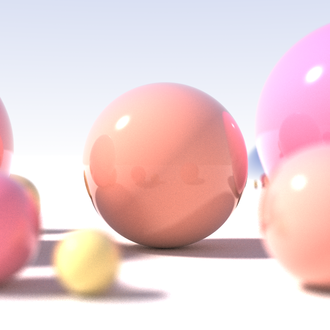
\includegraphics[width=7cm]{img/raytraced_depth_of_field.png}
			\end{center}%
			\caption{Depth of field in action. The camera lens is focused on the center sphere, making it appear sharp. The other spheres appear to be blurry.}%
			\label{fig:depth_of_field}%
		\end{figure}%

	\subsection{Motion blur}
		Motion blur is a camera effect that comes up when the camera or an object in the scene is moving while a picture is being taken. The camera requires itself and the objects in the scene to be still in order for light to hit the lens in focus. If the camera or an object is moving while the light is hitting the lens, then the light of the new scene will intersect the light of the old scene causing a blur. This effect can be easily rendered in screen space by taking into account in which direction the camera or the object is moving, as well as at what velocity, which can also be evaluated using the previous frame, and blurring accordingly \cite{MOB}.